\subsection{Bài tập trắc nghiệm}
% \BTTN
% \PHIEUTRACNGHIEM
\Opensolutionfile{ans}[ans/ans-2-B19]
\begin{ex}%[2D6N2-1]Câu 1
Cho hai biến cố $A$ và $B$ với $0<P(B)<1$. Khi đó công thức xác suất toàn phần cho biến cố $A$ là
	\choice
	{\True $\mathrm{P}(A)=\mathrm{P}(B)\mathrm{P}(A|B)+\mathrm{P}(\overline{B})\mathrm{P}(A|\overline{B})$}
	{$\mathrm{P}(A)=\mathrm{P}(A)\mathrm{P}(A|B)+\mathrm{P}(\overline{A})\mathrm{P}(A|\overline{B})$}
	{$\mathrm{P}(A)=\mathrm{P}(\overline{B})\mathrm{P}(A|B)+\mathrm{P}(B)\mathrm{P}(A|\overline{B})$}
	{$\mathrm{P}(B)=\mathrm{P}(\overline{B})\mathrm{P}(A|B)+\mathrm{P}(B)\mathrm{P}(B|\overline{B})$}
	\loigiai{Cho hai biến cố $A$ và $B$ với $0<P(B)<1$. Khi đó 
	$\mathrm{P}(A)=\mathrm{P}(B)P(A|B)+\mathrm{P}(\overline{B})\mathrm{P}(A|\overline{B})$ 
	gọi là {\bf công thức xác suất toàn phần}.
	}
\end{ex}

\begin{ex}%[2D6H2-1]Câu 2
Cho hai biến cố $A=A_1+A_2$ và biến cố $B=B_1+B_2$ biểu diễn theo đồ ven như sau
\begin{center}
\tikzset{every picture/.style={line width=0.75pt}} %set default line width to 0.75pt 
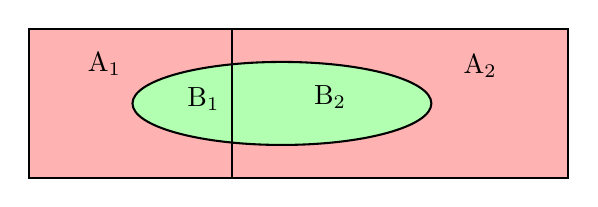
\begin{tikzpicture}[x=0.75pt,y=0.75pt,yscale=-1,xscale=1]
	%uncomment if require: \path (0,300); %set diagram left start at 0, and has height of 300
	%Shape: Rectangle [id:dp41068169978107316] 
	\draw [fill=red!30] (94,104) -- (354,104) -- (354,176) -- (94,176) -- cycle ;
	%Shape: Ellipse [id:dp24667066386593728] 
	\draw [fill=green!30] (144,140) .. controls (144,128.95) and (176.24,120) .. (216,120) .. controls (255.76,120) and (288,128.95) .. (288,140) .. controls (288,151.05) and (255.76,160) .. (216,160) .. controls (176.24,160) and (144,151.05) .. (144,140) -- cycle ;
	%Straight Lines [id:da2324528203840277] 
	\draw (192,104) -- (192,176) ;
	% Text Node
	\draw (302,115) node [anchor=north west][inner sep=0.75pt] [align=left] {A\textsubscript{2}};
	% Text Node
	\draw (121,114) node [anchor=north west][inner sep=0.75pt] [align=left] {A\textsubscript{1}};
	% Text Node
	\draw (169,131) node [anchor=north west][inner sep=0.75pt] [align=left] {B\textsubscript{1}};
	% Text Node
	\draw (230,130) node [anchor=north west][inner sep=0.75pt] [align=left] {B\textsubscript{2}};
\end{tikzpicture}
\end{center}
Tính xác xuất của $P(A)$.
	\choice
	{$\mathrm{P}(A)=\mathrm{P}(B_1)\mathrm{P}(A_1|B_1)+\mathrm{P}(B_2)\mathrm{P}(A_1|B_2)$}
	{\True $\mathrm{P}(A)=\mathrm{P}(B_1)\mathrm{P}(A|B_1)+\mathrm{P}(B_2)\mathrm{P}(A|B_2)$}
	{$\mathrm{P}(A)=\mathrm{P}(B)\mathrm{P}(A_1|B_1)+\mathrm{P}(B)\mathrm{P}(A_2|B_2)$}
	{$\mathrm{P}(A)=\mathrm{P}(A_1)\mathrm{P}(A|B_1)+\mathrm{P}(B_2)\mathrm{P}(A|B_2)$}
	\loigiai{ 
	Cho hai biến cố $A$ và $B$ với $0<P(B)<1$. Khi đó 
	$\mathrm{P}(A)=\mathrm{P}(B)\mathrm{P}(A|B)+\mathrm{P}(\overline{B})\mathrm{P}(A|\overline{B})$ 
	gọi là {\bf công thức xác suất toàn phần}.\\
	 $\Rightarrow \mathrm{P}(A)=\mathrm{P}(B_1)\mathrm{P}(A|B_1)+\mathrm{P}(B_2)\mathrm{P}(A|B_2)$}
\end{ex}

\begin{ex}%[2D6N2-1]Câu 3
Giả sử hai biến cố $A$ và $B$ ngẫu nhiên thỏa mãn $\mathrm{P}(A)>0$ với $0<\mathrm{P}(B)<1$. Khi đó công thức {\bf Bayes} là
	\choice
	{$\mathrm{P}(A|B)=\dfrac{\mathrm{P}(B)\mathrm{P}(A|B)}{\mathrm{P}(B)\mathrm{P}(A|B)+\mathrm{P}(\overline{B})\mathrm{P}(A|\overline{B})}$}
	{$\mathrm{P}(B|A)=\dfrac{\mathrm{P}(A)P(A|B)}{\mathrm{P}(B)\mathrm{P}(A|B)+\mathrm{P}(\overline{B})\mathrm{P}(A|\overline{B})}$}
	{\True $\mathrm{P}(B|A)=\dfrac{\mathrm{P}(B)P(A|B)}{\mathrm{P}(B)\mathrm{P}(A|B)+\mathrm{P}(\overline{B})\mathrm{P}(A|\overline{B})}$}
	{$\mathrm{P}(B|A)=\dfrac{\mathrm{P}(B)\mathrm{P}(B|A)}{\mathrm{P}(B)\mathrm{P}(A|B)+\mathrm{P}(\overline{B})\mathrm{P}(A|\overline{B})}$}
	\loigiai{Giả sử hai biến cố $A$ và $B$ ngẫu nhiên thỏa mãn $P(A)>0$ với $0<P(B)<1$. Khi đó\\
	$\mathrm{P}(B|A)=\dfrac{\mathrm{P}(B)\mathrm{P}(A|B)}{\mathrm{P}(B)P(A|B)+\mathrm{P}(\overline{B})\mathrm{P}(A|\overline{B})}$
	 gọi là công thức {\bf Bayes}. 
	}
\end{ex}

\begin{ex}%[2D6N2-2]
	Cho $\mathrm{P}(A)=\dfrac{2}{5}$; $\mathrm{P}(B \mid A)=\dfrac{1}{3}$; $\mathrm{P}(B \mid \overline{A})=\dfrac{1}{4}$. Giá trị của $\mathrm{P}(B)$ là 
	\choice
	{$\dfrac{19}{60}$}
	{\True $\dfrac{17}{60}$}
	{$\dfrac{9}{20}$}
	{$\dfrac{7}{30}$}
	\loigiai{
	Áp dụng công thức xác suất toàn phần ta có
	$$
	\mathrm{P}(B)=\mathrm{P}(A) \cdot \mathrm{P}(B \mid A)+\mathrm{P}\left(\overline{A}\right) \cdot \mathrm{P}(B \mid \overline{A})=\dfrac{2}{5} \cdot \dfrac{1}{3}+\dfrac{3}{5} \cdot \dfrac{1}{4}=\dfrac{17}{60}.
	$$
	}
\end{ex}

\begin{ex}%[2D6N2-2]
	Cho hai biến cố $A$, $B$ với $\mathrm{P}(B)=0{,}6$; $\mathrm{P}(A \mid B)=0{,}7$ và $\mathrm{P}(A \mid \overline{B})=0{,}4$. Khi đó, $\mathrm{P}(A)$ bằng 
	\choice
	{$0{,}7$}
	{$0{,}4$}
	{\True $0{,}58$}
	{$0{,}52$}
	\loigiai{
	Ta có $\mathrm{P}(\overline{B})=1-\mathrm{P}(B)=1-0{,}6=0{,}4$.\\
	Áp dụng công thức xác suất toàn phần, ta có
	$$
	\mathrm{P}(A)=\mathrm{P}(A \mid B) \cdot \mathrm{P}(B)+\mathrm{P}(A \mid \overline{B}) \cdot \mathrm{P}(\overline{B})=0{,}7 \cdot 0{,}6+0{,}4 \cdot 0{,}4=0{,}58.
	$$
	}
\end{ex}

\begin{ex}%[2D6N2-1]
	Theo công thức Bayes ta có 
	\choice
	{$\mathrm{P}(A \mid B)=\dfrac{\mathrm{P}(B)\cdot \mathrm{P}(B \mid A)}{\mathrm{P}(A)}$}
	{$\mathrm{P}(B \mid A)=\dfrac{\mathrm{P}(A)\cdot \mathrm{P}(B \mid A)}{\mathrm{P}(B)}$}
	{\True $\mathrm{P}(A \mid B)=\dfrac{\mathrm{P}(A)\cdot \mathrm{P}(B \mid A)}{\mathrm{P}(B)}$}
	{$\mathrm{P}(A \mid B)=\dfrac{\mathrm{P}(B)\cdot \mathrm{P}(A \mid B)}{\mathrm{P}(A)}$}
	\loigiai{
	Theo công thức Bayes ta có $\mathrm{P}(A \mid B)=\dfrac{\mathrm{P}(A)\cdot \mathrm{P}(B \mid A)}{\mathrm{P}(B)}$
	}
\end{ex}

\begin{ex}%[2D6N2-3]
	Cho $\mathrm{P}(A)=\dfrac{4}{5}$; $\mathrm{P}(B \mid A)=\dfrac{2}{3}$; $\mathrm{P}(B \mid \overline{A})=\dfrac{1}{4}$. Giá trị của $\mathrm{P}(A \mid B)$ là 
	\choice
	{$\dfrac{33}{35}$}
	{\True $\dfrac{32}{35}$}
	{$\dfrac{9}{35}$}
	{$\dfrac{26}{35}$}
	\loigiai{
	Áp dụng công thức Bayes ta có
	$$
	\mathrm{P}(A \mid B)=\dfrac{\mathrm{P}(A) \cdot \mathrm{P}(B \mid A)}{\mathrm{P}(A) \cdot \mathrm{P}(B \mid A)+\mathrm{P}(\overline{A}) \cdot \mathrm{P}(B \mid \overline{A})}=\dfrac{\dfrac{4}{5} \cdot \dfrac{2}{3}}{\dfrac{4}{5} \cdot \dfrac{2}{3}+\dfrac{1}{5} \cdot \dfrac{1}{4}}=\dfrac{32}{35}.
	$$
	}
\end{ex}

\begin{ex}%[2D6H2-2]
	Tỉ lệ người dân đã tiêm vắc xin phòng bệnh A ở một địa phương là $65 \%$. Trong số những người đã tiêm phòng, tỉ lệ mắc bệnh A là $5 \%$ còn trong số những người chưa tiêm, tỉ lệ mắc bệnh A là $17 \%$. Gặp ngẫu nhiên một người ở địa phương đó. Xác suất người đó mắc bệnh A là 
	\choice
	{$0{,}0325$}
	{$0{,}018$}
	{\True $0{,}092$}
	{$0{,}0525$}
	\loigiai{
	Gọi $H_1$ là biến cố \lq\lq  Gặp được người đã tiêm vắc xin phòng bệnh A\rq\rq, $H_2$ là biến cố \lq\lq  Gặp được người chưa tiêm vắc xin phòng bệnh A\rq\rq, $K$ là biến cố \lq\lq  Người đó mắc bệnh A\rq\rq. \\
	Theo công thức xác suất toàn phần, ta có
	\begin{eqnarray*}
	\mathrm{P}(K)&=&\mathrm{P}\left(H_1\right) \cdot \mathrm{P}\left(K \mid H_1\right)+\mathrm{P}\left(H_2\right) \cdot \mathrm{P}\left(K \mid H_2\right) \\
	&=& 0{,}65 \cdot 0{,}05+0{,}35 \cdot 0{,}17=0{,}092.
	\end{eqnarray*}
	}
\end{ex}

\begin{ex}%[2D6H2-2]
	Một nhà máy có hai phân xưởng I và II. Phân xưởng I sản xuất $40 \%$ số sản phẩm và phân xưởng II sản xuất $60 \%$ số sản phẩm. Tỉ lệ sản phẩm bị lỗi của phần xưởng I là $2 \%$ và của phân xưởng II là $1 \%$. Kiểm tra ngẫu nhiên $1$ sản phẩm của nhà máy và xác suất để sản phẩm đó bị lỗi là 
	\choice
	{$0{,}02$}
	{$0{,}6$}
	{\True $0{,}014$}
	{$0{,}01$}
	\loigiai{
	Gọi $A$ là biến cố \lq\lq  Sản phẩm bị lỗi\rq\rq, $B$ là biến cố \lq\lq  Sản phẩm lấy ra do phân xưởng $I$ sản xuất\rq\rq.\\
	Do phân xưởng I sản xuất $40 \%$ số sản phẩm và phân xưởng II sản xuất $60 \%$ số sản phẩm nên
	$$
	\mathrm{P}(B)=0{,}4 \,\,\text{và}\,\, \mathrm{P}(\overline{B})=1-0{,}4=0{,}6.
	$$
	Do tỉ lệ sản phẩm bị lỗi của phân xưởng I là $2 \%$ và của phân xưởng II là $1 \%$ nên
	$$
	\mathrm{P}(A \mid B)=0{,}02 \,\, \text{và} \,\, \mathrm{P}(A \mid \overline{B})=1-0{,}01.
	$$
	Xác suất để sản phẩm lấy ra bị lỗi là
	$$
	\mathrm{P}(A)=\mathrm{P}(B) \mathrm{P}(A \mid B)+\mathrm{P}(\overline{B}) \mathrm{P}(A \mid \overline{B})=0{,}4 \cdot 0{,}02+0{,}6 \cdot 0{,}01=0{,}014.
	$$
	}
\end{ex}

\begin{ex}%[2D6V2-4]
	Cho $A$, $B$ là các biến cố thỏa mãn $\mathrm{P}(\overline{A}\cap\overline{B})=0{,}35$; $\mathrm{P}(A)=0{,}25$; $\mathrm{P}(B)=0{,}6$. Giá trị của $\mathrm{P}(A|B)$ bằng
	\choice
	{$\dfrac{1}{5}$}
	{\True$\dfrac{1}{3}$}
	{$\dfrac{7}{15}$}
	{$\dfrac{2}{3}$}
	\loigiai{Ta có $\mathrm{P}(\overline{A}\cap\overline{B}) = \mathrm{P}\left( \overline A \right)\mathrm{P}\left( \overline B |\overline A \right) \Rightarrow \mathrm{P}\left( \overline B |\overline A \right) = \dfrac{\mathrm{P}(\overline{A}\cap\overline{B})}{\mathrm{P}\left( \overline A \right)} = \dfrac{0{,}35}{0{,}75} = \dfrac{7}{15}.$ \\
	Suy ra $\mathrm{P}\left( B|\overline A \right) = 1 - \dfrac{7}{{15}} = \dfrac{8}{{15}}$.\\
	Theo công thức xác suất toàn phần, ta có
	\begin{eqnarray*}
	&&\mathrm{P}\left( B \right) = \mathrm{P}\left( B|A \right)\mathrm{P}\left( A \right) + \mathrm{P}\left( B|\overline A \right)\mathrm{P}\left( \overline A\right)\\
	&\Rightarrow& \mathrm{P}\left(B|A\right) = \dfrac{\mathrm{P}\left( B \right) - \mathrm{P}\left( {B|\overline A } \right)\mathrm{P}\left( {\overline A } \right)}{\mathrm{P}\left( A \right)} = \dfrac{0{,}6 - \dfrac{8}{{15}} \cdot 0{,}75}{0{,}25} = 0{,}8.
	\end{eqnarray*}
	Theo công thức Bayes, ta được
	$$\mathrm{P}\left( A|B\right) = \dfrac{\mathrm{P}\left( A \right)\mathrm{P}\left( {B|A} \right)}{\mathrm{P}\left( B \right)} = \dfrac{0{,}25 \cdot 0{,}8}{0{,}6} = \dfrac{1}{3}.$$}
\end{ex}

\begin{ex}%[2D6H2-3]
	Một bệnh viện có hai phòng khám là phòng A và phòng B với khả năng lựa chọn của bệnh nhân là như nhau. Tỉ lệ bệnh nhân nam có ở phòng A và phòng B lần lượt là $60\%$ và $40\%$. Một người bệnh được chọn ngẫu nhiêu từ hai phòng khám và biết người này là nam, xác suất để người bệnh được chọn đến từ phòng A là
	\choice
	{\True $0{,}6$}
	{$0{,}5$}
	{$0{,}4$}
	{$0{,}3$}
	\loigiai{Một người bệnh được chọn ngẫu nhiên từ hai phòng khám.\\
	Gọi $X$ là biến cố \lq \lq Người đó đến từ phòng khám A\rq \rq \, và $Y$, $\overline{Y}$ lần lượt là biến cố \lq \lq Người đó là nam\rq \rq \; và \lq \lq Người đó không là nam\rq \rq.\\
	Ta có sơ đồ hình cây sau
	\begin{center}
	\begin{tikzpicture}[>=stealth,scale=0.6]
	%Khung 1
	\draw (-2,-1) rectangle (2.2,0);
	\draw (0.1,-0.5) node{Bệnh nhân được chọn} ;
	%Mui ten 1,2
	\draw [->] (2.2,-0.5)--(3.8,1.6) node[pos=0.5,sloped,above]{$0{,}5$};
	\draw [->] (2.2,-0.5)--(3.8,-2.6) node[pos=0.5,sloped,below]{$0{,}5$};
	%Khung 2.1
	\draw (3.8,1.1) rectangle (5.1,2.1);
	\draw (8.9/2,1.6) node{$X$} ;
	%Khung 2.2
	\draw (3.8,-2.1) rectangle (5.1,-3.1);
	\draw (8.9/2,-2.6) node{$\overline{X}$} ;
	%Mui ten 3,4
	\draw [->] (5.1,1.6)--(6.5,2.6) node[pos=0.5,sloped,above]{$0{,}6$};
	\draw [->] (5.1,1.6)--(6.5,0.6) node[pos=0.5,sloped,below]{$0{,}4$};
	%Mui ten 5,6
	\draw [->] (5.1,-2.6)--(6.5,-1.6) node[pos=0.5,sloped,above]{$0{,}4$};
	\draw [->] (5.1,-2.6)--(6.5,-3.6) node[pos=0.5,sloped,below]{$0{,}6$};
	%Khung 3.1
	\draw (6.5,2.2) rectangle (7.7,3.2);
	\draw (7.1,5.4/2) node{$Y$} ;
	%Khung 3.2
	\draw (6.5,1.2) rectangle (7.7,0.2);
	\draw (7.1,1.4/2) node{$\overline{Y}$} ;
	%Khung 3.3
	\draw (6.5,-1.1) rectangle (7.7,-2.1);
	\draw (7.1,-3.2/2) node{$Y$} ;
	%Khung 3.3
	\draw (6.5,-2.9) rectangle (7.7,-3.9);
	\draw (7.1,-3.4) node{$\overline{Y}$} ;
	%Kết quả
	\draw (9.5,3.7) node{\textbf{Kết quả}};	
	\draw (9.5,2.7) node{$XY$};
	\draw (9.5,0.7) node{$X \overline{Y}$};
	\draw (9.5,-1.6) node{$\overline{X}Y$};
	\draw (9.5,-3.4) node{$\overline{X}\overline{Y}$};
	%Xác suất
	\draw (12.5,3.7) node{\textbf{Xác suất}};	
	\draw (12.5,2.7) node{$0{,}3$};
	\draw (12.5,0.7) node{$0{,}2$};
	\draw (12.5,-1.6) node{$0{,}2$};
	\draw (12.5,-3.4) node{$0{,}3$};	
	\end{tikzpicture}
	\end{center}
	Theo công thức Bayes, ta có $$\mathrm{P}(X|Y)=\dfrac{\mathrm{P}(X)\mathrm{P}(Y|X)}{\mathrm{P}(X)\mathrm{P}(Y|X)+\mathrm{P}(\overline{X})\mathrm{P}(Y|\overline{X})}=\dfrac{0{,}3}{0{,}3+0{,}2}=0{,}6.$$
	Vậy với một người bệnh được chọn ngẫu nhiêu từ hai phòng khám và biết người này là nam, xác suất để người đó đến từ phòng A là $0{,}6$.}
\end{ex}

\begin{ex}%[2D6V2-3]
	Một bệnh viện đang xét nghiệm cho một số bệnh nhân để xác định liệu họ có nhiễm virus $X$ hay không. Xác suất để một bệnh nhân bị nhiễm virus $X$ là $0{,}05$. Khi xét nghiệm, nếu một bệnh nhân bị nhiễm thì xác suất để kết quả xét nghiệm dương tính là $0{,}95$. Nếu một bệnh nhân không bị nhiễm thì xác suất để kết quả xét nghiệm âm tính là $0{,}98$. Một bệnh nhân được chọn ngẫu nhiên và có kết quả xét nghiệm dương tính. Xác suất để bệnh nhân đó thực sự bị nhiễm virus $X$ là
	\choice
	{$\dfrac{133}{2000}$}
	{$\dfrac{19}{400}$}
	{\True $\dfrac{5}{7}$}
	{$\dfrac{2}{7}$}
	\loigiai{Một bệnh nhân đến một bệnh viên để xét nghiệm.\\
	Gọi $A$ là biến cố \lq \lq Bệnh nhân bị nhiễm virus $X$\rq \rq \, và $B$, $\overline{B}$ lần lượt là biến cố \lq \lq Kết quả xét nghiệm dương tính\rq \rq \; và \lq \lq Kết quả xét nghiệm âm tính\rq \rq.\\
	Ta xét sơ đồ hình cây như sau
	\begin{center}
	\begin{tikzpicture}[>=stealth,scale=0.6]
	%Khung 1
	\draw (-3.5,-1) rectangle (2.2,0);
	\draw (-1.3/2,-0.5) node{Bệnh nhân được xét nghiệm} ;
	%Mui ten 1,2
	\draw [->] (2.2,-0.5)--(3.8,1.6) node[pos=0.5,sloped,above]{$0{,}05$};
	\draw [->] (2.2,-0.5)--(3.8,-2.6) node[pos=0.5,sloped,below]{$0{,}95$};
	%Khung 2.1
	\draw (3.8,1.1) rectangle (5.1,2.1);
	\draw (8.9/2,1.6) node{$A$} ;
	%Khung 2.2
	\draw (3.8,-2.1) rectangle (5.1,-3.1);
	\draw (8.9/2,-2.6) node{$\overline{A}$} ;
	%Mui ten 3,4
	\draw [->] (5.1,1.6)--(6.5,2.6) node[pos=0.5,sloped,above]{$0{,}95$};
	\draw [->] (5.1,1.6)--(6.5,0.6) node[pos=0.5,sloped,below]{$0{,}05$};
	%Mui ten 5,6
	\draw [->] (5.1,-2.6)--(6.5,-1.6) node[pos=0.5,sloped,above]{$0{,}02$};
	\draw [->] (5.1,-2.6)--(6.5,-3.6) node[pos=0.5,sloped,below]{$0{,}98$};
	%Khung 3.1
	\draw (6.5,2.2) rectangle (7.7,3.2);
	\draw (7.1,5.4/2) node{$B$} ;
	%Khung 3.2
	\draw (6.5,1.2) rectangle (7.7,0.2);
	\draw (7.1,1.4/2) node{$\overline{B}$} ;
	%Khung 3.3
	\draw (6.5,-1.1) rectangle (7.7,-2.1);
	\draw (7.1,-3.2/2) node{$B$} ;
	%Khung 3.3
	\draw (6.5,-2.9) rectangle (7.7,-3.9);
	\draw (7.1,-3.4) node{$\overline{B}$} ;
	%Kết quả
	\draw (9.5,3.7) node{\textbf{Kết quả}};	
	\draw (9.5,2.7) node{$AB$};
	\draw (9.5,0.7) node{$A\overline{B}$};
	\draw (9.5,-1.6) node{$\overline{A}B$};
	\draw (9.5,-3.4) node{$\overline{A}\cap\overline{B}$};
	%Xác suất
	\draw (12.5,3.7) node{\textbf{Xác suất}};	
	\draw (12.5,2.7) node{$0{,}0475$};
	\draw (12.5,0.7) node{$0{,}0025$};
	\draw (12.5,-1.6) node{$0{,}019$};
	\draw (12.5,-3.4) node{$0{,}931$};
	\end{tikzpicture}
	\end{center}
	Theo công thức Bayes, ta có $$\mathrm{P}(A|B)=\dfrac{\mathrm{P}(A)\mathrm{P}(B|A)}{\mathrm{P}(A)\mathrm{P}(B|A)+\mathrm{P}(\overline{A})\mathrm{P}(B|\overline{A})}=\dfrac{0{,}0475}{0{,}0475+0{,}019}=\dfrac{5}{7}.$$	 
	Vậy với một bệnh nhân có kết quả xét nghiệm dương tính, xác suất để bệnh nhân đó thực sự bị nhiễm virus $X$ là $\dfrac{5}{7}$.}
\end{ex}

\begin{ex}%[2D6V2-2]
	Kết quả khảo sát tại một xã cho thấy có $20 \%$ cư dân hút thuốc lá. Tỉ lệ cư dân thường xuyên gặp các vấn đề sức khoẻ về đường hô hấp trong số những người hút thuốc lá và không hút thuốc lá lần lượt là $70 \%$, $15 \%$. Tỉ lệ gặp một cư dân của xã thì xác suất người đó thường xuyên gặp các vấn đề sức khoẻ về đường hô hấp là bao nhiêu phần trăm? 
	\choice
	{\True $26 \%$}
	{$12 \%$}
	{$68 \%$}
	{$24 \%$}
	\loigiai{
	Giả sử ta gặp một cư dân của xã, gọi $A$ là biến cố \lq\lq  Người đó có hút thuốc lá\rq\rq\, và $B$ là biến cố \lq\lq  Người đó thường xuyên gặp các vấn đề sức khoẻ về đường hô hấp\rq\rq. Ta có sơ đồ hình cây sau.
	\begin{center}
	\begin{tikzpicture}[scale=.3,>=stealth,every node/.style={shape=rectangle,draw,rounded corners, color=blue, fill=blue!10}]
	%-------------
	\tikzstyle{block} = [rectangle, draw, fill=blue!10, rounded corners, text centered, text width = 10em, minimum height = 2em]
	%-------------
	\node (c1) {Gặp một cư dân};
	\node (c2) [above right = 2cm of c1]{$A$};
	\node (c3) [ below right= 2cm of c1]{$\overline{A}$};
	\node (c4) [above right = 1cm of c2]{$B$} ;
	\node (c5) [below right = 1cm of c2]{$\overline{B}$};
	\node (c6) [ above right =1cm of c3]{$B$};
	\node (c7) [ below right = 1cm of c3]{$\overline{B}$};
	%--------------
	\draw 
	(17.5,15) node[right] {\text{Kết quả}} 
	(20,11.3) node[right] {$AB$} 
	(20,2.5) node[right] {$A\overline{B}$} 
	(20,-2.5) node[right] {$\overline{A}B$} 
	(20,-11.5) node[right] {$\overline{A}\cap \overline{B}$};
	%--------------
	\draw 
	(25,15) node[right] {\text{Xác suất}} 
	(25,11.3) node[right] {$0{,}14$} 
	(25,2.5) node[right] {$0{,}06$} 
	(25,-2.5) node[right] {$0{,}12$} 
	(25,-11.5) node[right] {$0{,}68$};
	%------------
	\draw[->] (c1.east) --node[above left]{$0{,}2$} (c2.west);
	\draw[->] (c1.east) --node[below left]{$0{,}8$} (c3.west);
	\draw[->] (c2.east) --node[above left]{$0{,}7$} (c4.west);
	\draw[->] (c2.east) --node[below left]{$0{,}3$} (c5.west);
	\draw[->] (c3.east) --node[above left]{$0{,}15$} (c6.west);
	\draw[->] (c3.east) -- node[below left]{$0{,}85$} (c7.west);
	\end{tikzpicture}
	\end{center}
	Ta có $\mathrm{P}(B)=\mathrm{P}(A) \cdot \mathrm{P}(B | A)+\mathrm{P}(\overline{A}) \cdot \mathrm{P}\left(B | \overline{A}\right)=0{,}14+0{,}12=0{,}26$.\\
	Vậy nếu ta gặp một cư dân của xã thì xác suất người đó thường xuyên gặp các vấn đề sức khoẻ về đường hô hấp là $26\%$.
	}
\end{ex}

\begin{ex}%[2D6V2-3]
	Ở một địa phương $X$, xác suất để một người lớn trên $40$ tuổi mắc bệnh ung thư là $0{,}05$. Xác suất bác sĩ chẩn đoán đúng một người mắc bệnh ung thư là $0{,}78$ và chẩn đoán sai (không bị ung thư nhưng được chẩn đoán mắc bệnh) là $0{,}06$. Xác suất để một người thật sự mắc bệnh ung thư khi nhận được kết quả chẩn đoán bị ung thư bằng
	\choice
	{\True$0{,}40625$}
	{$0{,}096$}
	{$0{,}904$}
	{$0{,}59375$}
	\loigiai{Một bệnh nhân trên 40 tuổi ở địa phương X đến bác sĩ để khám bệnh ung thư.\\
	Gọi $A$ là biến cố \lq \lq Người đó mắc bệnh ung thư\rq \rq \, và $B$, $\overline{B}$ lần lượt là biến cố \lq \lq Bác sĩ chẩn đoán người đó bị ung thư\rq \rq \;và \lq \lq Bác sĩ chẩn đoán người đó không bị ung thư\rq \rq.\\
	Ta xét sơ đồ hình cây như sau
	\begin{center}
	\begin{tikzpicture}[>=stealth,scale=0.7]
	%Khung 1
	\draw (-3.5,-1) rectangle (2.2,0);
	\draw (-1.3/2,-0.5) node{Bệnh nhân được chẩn đoán} ;
	%Mui ten 1,2
	\draw [->] (2.2,-0.5)--(3.8,1.6) node[pos=0.5,sloped,above]{$0{,}05$};
	\draw [->] (2.2,-0.5)--(3.8,-2.6) node[pos=0.5,sloped,below]{$0{,}95$};
	%Khung 2.1
	\draw (3.8,1.1) rectangle (5.1,2.1);
	\draw (8.9/2,1.6) node{$A$} ;
	%Khung 2.2
	\draw (3.8,-2.1) rectangle (5.1,-3.1);
	\draw (8.9/2,-2.6) node{$\overline{A}$} ;
	%Mui ten 3,4
	\draw [->] (5.1,1.6)--(6.5,2.6) node[pos=0.5,sloped,above]{$0{,}78$};
	\draw [->] (5.1,1.6)--(6.5,0.6) node[pos=0.5,sloped,below]{$0{,}22$};
	%Mui ten 5,6
	\draw [->] (5.1,-2.6)--(6.5,-1.6) node[pos=0.5,sloped,above]{$0{,}06$};
	\draw [->] (5.1,-2.6)--(6.5,-3.6) node[pos=0.5,sloped,below]{$0{,}94$};
	%Khung 3.1
	\draw (6.5,2.2) rectangle (7.7,3.2);
	\draw (7.1,5.4/2) node{$B$} ;
	%Khung 3.2
	\draw (6.5,1.2) rectangle (7.7,0.2);
	\draw (7.1,1.4/2) node{$\overline{B}$} ;
	%Khung 3.3
	\draw (6.5,-1.1) rectangle (7.7,-2.1);
	\draw (7.1,-3.2/2) node{$B$} ;
	%Khung 3.3
	\draw (6.5,-2.9) rectangle (7.7,-3.9);
	\draw (7.1,-3.4) node{$\overline{B}$} ;
	%Kết quả
	\draw (9.5,3.7) node{\textbf{Kết quả}};	
	\draw (9.5,2.7) node{$AB$};
	\draw (9.5,0.7) node{$A\overline{B}$};
	\draw (9.5,-1.6) node{$\overline{A}B$};
	\draw (9.5,-3.4) node{$\overline{A}\cap\overline{B}$};
	%Xác suất
	\draw (12.5,3.7) node{\textbf{Xác suất}};	
	\draw (12.5,2.7) node{$0{,}039$};
	\draw (12.5,0.7) node{$0{,}011$};
	\draw (12.5,-1.6) node{$0{,}057$};
	\draw (12.5,-3.4) node{$0{,}893$};
	\end{tikzpicture}
	\end{center}
	Theo công thức Bayes, ta có $$\mathrm{P}(A|B)=\dfrac{\mathrm{P}(A)\mathrm{P}(B|A)}{\mathrm{P}(A)\mathrm{P}(B|A)+\mathrm{P}(\overline{A})\mathrm{P}(B|\overline{A})}=\dfrac{0{,}039}{0{,}039+0{,}057}=0{,}40625.$$	 
	Vậy xác suất để một người thật sự mắc bệnh ung thư khi nhận được kết quả chẩn đoán bị ung thư bằng $0{,}40625$.}
\end{ex}

\begin{ex}%[2D6V2-2]
	Trung tâm kiểm soát và phòng ngừa dịch bệnh Hoa Kỳ (Centers for Disease Control and Prevention, viết tắt là (CDC) thống kê vào thời điểm năm $2020 - 2021$ về số lượng sốc phản vệ sau khi tiêm vaccine ở một số nơi tại Hoa Kỳ và châu Âu như sau: Trong $360{,}19$ triệu liều vaccine $P$ được sử dụng có $581$ ca sốc phản vệ (có khả năng gây tử vong) và $4\,259$ ca phản ứng phụ (không sốc phản vệ, không gây tử vong); trong $67{,}72$ triệu liều vaccine $A$ được sử dụng có $195$ ca sốc phản vệ và $1\,118$ ca phản ứng phụ.\\
	\textit{(Nguồn: https://www.ncbi.nlm.nih.gov/pmc/articles/PMC8626274/)}
	\choice
	{$1{,}9 \cdot 10^{-6}$}
	{$2{,}8 \cdot 10^{-6}$}
	{\True $1{,}81 \cdot 10^{-6}$}
	{$2{,}81 \cdot 10^{-6}$}
	\loigiai{
	Xét ngẫu nhiên một người trong số được thống kê ở trên. Tính xác suất để người đó thuộc trường hợp sốc phản vệ (có khả năng gây tử vong).\\
	Gọi $X$ là biến cố “Người được chọn tiêm vaccine $P$”, khi đó $\overline X $ là biến cố “Người được chọn tiêm vaccine $A$”.\\
	$Y$ là biến cố “Người được chọn thuộc trường hợp sốc phản vệ”.\\
	Khi đó, xác suất chọn được người tiêm vaccine $P$ là $\mathrm{P}(X)=\dfrac{360{,}19 \cdot 10^6}{360{,}19 \cdot 10^6+67{,}72 \cdot 10^6}$.\\
	Xác suất chọn được người tiêm vaccine $A$ là $\mathrm{P}(\overline X)=\dfrac{67{,}72 \cdot 10^6}{360{,}19 \cdot 10^6+67{,}72 \cdot 10^6}$.\\
	Xác suất chọn được người bị sốc phản vệ, nếu người đó tiêm vaccine $P$ là $\mathrm{P}(Y|X)=\dfrac{581}{360{,}19 \cdot 10^6}$.\\
	Xác suất chọn được người bị sốc phản vệ, nếu người đó tiêm vaccine $A$ là $\mathrm{P}(Y|\overline X)=\dfrac{195}{67{,}72 \cdot 10^6}$.\\
	Áp dụng công thức tính xác suất toàn phần, ta có:
	$$\mathrm{P}(Y)=\mathrm{P}(X)\cdot \mathrm{P}(Y|X)+\mathrm{P}(\overline{X})\cdot \mathrm{P}(Y|\overline{X}) \approx 1{,}81 \cdot 10^{-6}.$$
	}
\end{ex}

\begin{ex}%[2D6V2-2]Câu 4
	Trên bàn có hai hộp $B_1$ và $B_2$ đều đựng đá cẩm thạch. Hộp $B_1$ chứa 7 viên xanh và 4 viên trắng. Hộp $B_2$ chứa 3 viên xanh và 10 viên vàng. Các hộp được sắp xếp sao cho xác suất chọn hộp $B_1$ là $\dfrac{1}{3}$ và xác suất chọn hộp $B_2$ là $\dfrac{2}{3}$. Kathy bị bịt mắt và dược yêu cầu chọn một viên đá cẩm thạch. Cô ấy sẽ được thưởng một chiếc TV nếu chọn được một viên màu xanh. Xác suất cô ấy được thưởng một chiếc TV màu xanh là bao nhiêu
	\choice
	{\True $\dfrac{157}{429}$}
	{$\dfrac{158}{429}$}
	{$\dfrac{159}{429}$}
	{$\dfrac{59}{429}$}
	\loigiai{Gọi $A$ là biến cố \lq\lq  Kathy được thưởng một chiếc TV\rq\rq.\\
	Gọi $B_j$ là biến cố \lq\lq  hộp $B_j$ được chọn\rq\rq, $j=1,2$.\\
	Xác suất $\mathrm{P}(B_1)=\dfrac{1}{3}, P(B_2)=\dfrac{2}{3}$.\\
	Xác suất cần tìm là \\ $\mathrm{P}(A)=\mathrm{P}(B_1)\cdot \mathrm{P}(A|B_1)+\mathrm{P}(B_2)\cdot \mathrm{P}(A|B_2)=\dfrac{1}{3}\cdot\dfrac{7}{11}+\dfrac{2}{3}\cdot\dfrac{3}{13}=\dfrac{157}{429}$.
	}
\end{ex}

\begin{ex}%[2D6V2-2]Câu 5
Có $0{,}5\%$ dân số mắc bệnh $X$. Có một xét nghiệm để phát hiện bệnh $X$. Đối với những người mắc bệnh $X$, Xác suất xét nghiệm này không dương tính là $2\%$. Đối vơi những người không mắc bệnh $X$, xác suất xét nghiệm này dương tính là $3\%$. Xác suất một người được chọn ngẫu nhiên có kết quả dương tính với xét nghiệm phát hiện bệnh $X$ là bao nhiêu?
	\choice
	{$\dfrac{13}{400}$}
	{\True $\dfrac{139}{4000}$}
	{$\dfrac{137}{4000}$}
	{$\dfrac{13}{200}$}
	\loigiai{ Gọi $A$ là biến cố \lq\lq  người được chọn có kết quả dương tính với xét nghiệm phát hiện bệnh $X$ \rq\rq .\\
	Gọi $B_1$, $B_2$ lần lượt là biến cố \lq\lq  người được chọn mắc bệnh $X$\rq\rq. \\
	Xác suất $\mathrm{P}(B_1)=\dfrac{5}{1000}$, $\mathrm{P}(B_2)=\dfrac{995}{1000}$.\\
	Xác suất cần tìm là \\ $\mathrm{P}(A)=\mathrm{P}(B_1)\cdot \mathrm{P}(A|B_1)+\mathrm{P}(B_2)\cdot\mathrm{P}(A|B_2)=\dfrac{5}{1000}\cdot\dfrac{98}{1000}+\dfrac{995}{1000}\cdot\dfrac{3}{1000}=\dfrac{139}{4000}$
	}
\end{ex}

\begin{ex}%[2D6V2-2]Câu 6
Một cặp sinh đôi có thể do cùng một trứng sinh ra (sinh đôi thật), hoặc do hai trứng
khác nhau sinh ra (sinh đôi giả). Các cặp sinh đôi thật luôn cùng giới tính. Đối với
cặp sinh đôi giả thì khả năng cùng giới tính và khác giới tính là như nhau. Thống kê
cho thấy $34\%$ cặp sinh đôi đều là trai, $30\%$ cặp sinh đôi đều là gái, và $36\%$ cặp sinh đôi có giới tính khác nhau. Tìm xác suất sinh đôi thật?
	\choice
	{$0{,}29$}
	{$0{,}27$}
	{\True$0{,}28$}
	{$0{,}3$}
	\loigiai{Gọi $B_1$, $B_2$, $A$ lần lượt là biến cố \lq\lq  cặp sinh đôi là thật\rq\rq,\, \lq\lq  cặp sinh đôi là giả\rq\rq,\, \lq\lq  cặp sinh đôi cùng giới\rq\rq.
	\begin{eqnarray*}
	\mathrm{P}(A)& =& \mathrm{P}(B_1)\cdot \mathrm{P}(A|B_1)+\mathrm{P}(B_2)\mathrm{P}(A|B_2)\\
\Leftrightarrow	\, \, \, 0{,}34+0{,}3	&= & P(B_1)\cdot1+[1-P(B_1)]\cdot0{,}5\\
	\Rightarrow \quad \quad P(B_1) &= & 0{,28}
	\end{eqnarray*}
	}
\end{ex}

\begin{ex}%[2D6V2-2]Câu 7
	Một lô hạt giống được chia làm $2$ loại: loại $1$ chiếm $\dfrac{2}{3}$ số hạt của lô, còn lại là loại $2$. Hạt trong loại $1$ có tỉ lệ nảy mầm là $80\%$, loại $2$ có tỉ lệ nảy mầm là $60\%$. Hỏi tỉ lệ nảy mầm chung của lô hạt giống này là bao nhiêu? (Hay nói cách khác: Ta lấy ngẫu nhiên từ lô ra $1$ hạt giống. Tìm xác suất để chọn được hạt nảy mầm).
	\choice
	{$\dfrac{11}{16}$}
	{$\dfrac{11}{14}$}
	{$\dfrac{11}{11}$}
	{\True$\dfrac{11}{15}$}
	\loigiai{ Gọi $A_i$ là biến cố \lq\lq  hạt giống được lấy ra từ lô thứ $i$\rq\rq \, (với $i=1,2$).\\
	Gọi $A$ là biến cố \lq\lq  hạt giống được lấy ra là hạt nảy mầm\rq\rq .
	Dễ thấy rằng $A_1$, $A_2$, $A_3$ tạo thành một hệ đầy đủ các biến cố.\\
	Theo đề bài: $\mathrm{P}(A_1)=\dfrac{2}{3}$, $\mathrm{P}(A_2)=\dfrac{1}{3}$ và $\mathrm{P}(A|A_1)=0{,}8$, $\mathrm{P}(A|A_2)=0{,}6$.\\
	Áp dụng công thức xác suất đầy đủ
	$$\mathrm{P}(A)=\mathrm{P}(A_1)\cdot \mathrm{P}(A|A_1)+\mathrm{P}(A_2)\mathrm{P}(A|A_2)=\dfrac{2}{3}\cdot0{,}8+\dfrac{1}{3}\cdot0{,}6=\dfrac{11}{15}.$$
	}
\end{ex}

\begin{ex}%[2D6V2-2]Câu 8
Một trạm cấp cứu có $80\%$ nạn nhân bỏng nóng và $20\%$ bỏng do hóa chất. Loại bỏng do nóng có $30\%$ biến chứng và bỏng do hóa chất có $50\%$ biến chứng. Tìm xác suất của nạn nhân bị biến chứng.
	\choice
	{$0{,}35$}
	{$0{,}36$}
	{\True $0{,}34$}
	{$0{,}37$}
	\loigiai{ Gọi $A$ là biến cố \lq\lq  nạn nhân bị biến chứng\rq\rq.
	Gọi $A_1$ là biến cố \lq\lq  nạn nhân bị bỏng do nóng\rq\rq.
	Gọi $A_2$ là biến cố \lq\lq  nạn nhân bị bỏng do hóa chất\rq\rq .
	Ta thấy rằng $A_1$ và $A_2$ lập thành một hệ đầy đủ.\\
	Theo đề bài	$\mathrm{P}(A_1)=0{,}8$;\, $\mathrm{P}(A_2)=0{,}2$; \,$\mathrm{P}(A|A_1)=0{,}3$; \,$\mathrm{P}(A|A_2)=0{,}5$.\\
	Sử dụng công thức xác suất đầy đủ
	$$\mathrm{P}(A)=\mathrm{P}(A_1)\mathrm{P}(A|A_1)+P(A_2)\mathrm{P}(A|A_2)=0{,}8\cdot0{,}3+0{,}2\cdot0{,}5=0{,}34.$$
	}
\end{ex}

\begin{ex}%[2D6C2-2]Câu 9
Chuồng gà thứ nhất có $9$ con mái và $1$ con trống. Chuồng gà thứ hai có $1$ con mái và $5$ con trống. Từ mỗi chuồng gà bắt ra ngẫu nhiên một con. Các con gà còn lại được dồn vào chuồng thứ ba. Bắt ngẫu nhiên một con gà trong chuồng thứ ba. Tính xác suất để bắt được gà trống.
	\choice
	{$\dfrac{38}{107}$}
	{\True$\dfrac{38}{105}$}
	{$\dfrac{38}{109}$}
	{$\dfrac{39}{105}$}
	\loigiai{ 
	$B_1$ là biến cố $2$ con gà được bắt đều là trống.\\
	$B_2$ là biến cố $2$ con gà được bắt đều là mái.\\
	$B_3$ là biến cố $2$ con gà được bắt gồm $1$ trống và $1$ mái.\\
	$A$ là biến cố bắt được gà trống ở chuồng thứ ba.\\
	 $B_1$ xảy ra $\Rightarrow$ Chuồng thứ ba gồm: $10$ gà mái và $4$ gà trống.\\
	 $B_2$ xảy ra $\Rightarrow$ Chuồng thứ ba gồm: $8$ gà mái và $6$ gà trống.\\
	 $B_3$ xảy ra $\Rightarrow$ Chuồng thứ ba gồm: $9$ gà mái và $5$ gà trống.\\
	$\mathrm{P}(B_1)=\dfrac{1}{10}\cdot \dfrac{\mathrm{C}_{5}^{1}}{6}=\dfrac{1}{12}$;
	$\mathrm{P}(B_2)=\dfrac{\mathrm{C}_{9}^{1}}{10}\cdot \dfrac{1}{6}=\dfrac{3}{20}$;
	$\mathrm{P}(B_3)=1-\mathrm{P}(B_1)-\mathrm{P}(B_2)=\dfrac{23}{30}$.\\
	Xác suất để bắt được gà trống ở chuồng thứ ba là
	\begin{eqnarray*}
	\mathrm{P}(A)&=& \mathrm{P}(B_1)\mathrm{P}(A|B_1)+\mathrm{P}(B_2)\mathrm{P}(A|B_2)+\mathrm{P}(B_3)\mathrm{P}(A|B_3)\\
	&=& \dfrac{1}{12}\cdot\dfrac{4}{14}+\dfrac{3}{20}\cdot\dfrac{6}{14}+\dfrac{23}{30}\cdot\dfrac{5}{14}\\
	&= & \dfrac{38}{105}.
	\end{eqnarray*}
	}
\end{ex}

\begin{ex}%[2D6V2-3]Câu 10
Dây chuyền lắp ráp được các chi tiết do hai máy sản xuất. Trung bình máy thứ nhất cung cấp $60\%$ chi tiết, máy thứ hai cung cấp $40\%$ chi tiết. Khoảng $90\%$ chi tiết do máy thứ nhất sản xuất là đạt tiêu chuẩn, còn $85\%$ chi tiết do máy thứ hai sản xuất là đạt tiêu chuẩn. Lấy ngẫu nhiên từ dây chuyền một sản phẩm, lấy nó đạt tiêu chuẩn. Tìm xác suất để sản phẩm đó do máy thứ nhất sản xuất.
	\choice
	{$0{,}713$}
	{$0{,}715$}
	{$0{,}814$}
	{\True$0{,}614$}
	\loigiai{Gọi $A$ là biến cố \lq\lq  Chi tiết lấy từ dây chuyền đạt tiêu chuẩn\rq\rq.\\ $B_1$ là biến cố \lq\lq  Chi tiết do máy thứ nhất sản xuất \rq\rq.\\
	$B_2$ là biến cố \lq\lq  Chi tiết do máy thứ 2 sản xuất \rq\rq.\\
	Ta cần tính xác suất $\mathrm{P}(B_1|A)$.\\
	Theo điều kiện bài toán $\mathrm{P}(B_1)=0{,}6$; $\mathrm{P}(B_2)=0{,}4$; $\mathrm{P}(A|B_1)=0{,}9$; $\mathrm{P}(A|B_2)=0{,}85$. \\
	 Theo công thức Bayes
	 $$\mathrm{P}(B_1|A)=\dfrac{\mathrm{P}(B_1)\mathrm{P}(A|B_1)}{\mathrm{P}(B_1)\mathrm{P}(A|B_1)+\mathrm{P}(B_2)\mathrm{P}(A|B_2)}=\dfrac{0{,}6\cdot0{,9}}{0{,}6\cdot0{,9}+0{,}4\cdot0{,}85}=0{,}614.$$
	}
\end{ex}

\begin{ex}%[2D6C2-3]Câu 11
 Tan giờ học buổi chiều một sinh viên có $60\%$ về nhà ngay, nhưng do giờ cao điểm nên có $30\%$ ngày bị tắc đường nên bị về nhà muộn (từ $30$ phút trở lên) còn $20\%$ số ngày sinh viên đó vào quán Internet cạnh trường để chơi game, những ngày này xác suất về nhà muộn là $80\%$. Còn lại những ngày khác sinh viên đó đi chơi với bạn bè có xác suất về muộn là $90\%$. Tính xác suất sinh viên đó đi chơi với bạn và về muộn.
	\choice
	{$0{,}275$}
	{$0{,}575$}
	{\True $0{,}375$}
	{$0{,}475$}
	\loigiai{ 
	Gọi $B$ là biến cố sinh viên đi học về muộn \\
	Gọi $\overline{B}$ là biến cố sinh viên đó đi học không về muộn\\
	$E_1$ là biến cố tan học về nhà ngay $\Rightarrow \mathrm{P}(E_1)=0{,}6$; $\mathrm{P}(B|E_1)=0{,}3$.\\
 	$E_2$ là biến cố tan học đi chơi game $\Rightarrow \mathrm{P}(E_2)=0{,}2$; $\mathrm{P}(B|E_2)=0{,}8$.\\
	 $E_3$ là biến cố tan học về đi chơi với bạn $\Rightarrow \mathrm{P}(E_3)=0{,}2$; $\mathrm{P}(B|E_3)=0{,}9$.\\
	$B$ có thể xảy ra một trong 3 biến cố
	 \begin{eqnarray*}
	 	\mathrm{P}(B)&= & \mathrm{P}(E_1)\cdot \mathrm{P}(B|E_1)+\mathrm{P}(E_2)\cdot \mathrm{P}(B|E_2)+\mathrm{P}(E_3)\cdot \mathrm{P}(B|E_3)\\
	 	&= & 0{,}6\cdot0{,}3+0{,}2\cdot0{,}8+0{,}2\cdot0{,}9\\
	 	&= & 0{,}52.
	 \end{eqnarray*}
	Xác suất để sinh viên đó đi chơi với bạn và về muộn là
	$\mathrm{P}(E_3|B)=\dfrac{\mathrm{P}(E_3)\cdot \mathrm{P}(B|E_3)}{\mathrm{P}(B)}=0{,}375$.
	}
\end{ex}

\begin{ex}%[2D6V2-3]Câu 12
	Dây chuyền lắp ráp máy vô tuyến điện gồm các linh kiện là sản phẩm từ $2$ nhà máy sản xuất ra. Số linh kiện nhà máy $1$ sản xuất chiếm $55\%$, số linh kiện nhà máy $2$ sản xuất chiếm $45\%$; tỷ lệ sản phẩm đạt tiêu chuẩn của nhà máy $1$ là $90\%$, nhà máy $2$ là $87\%$. Lấy ngẫu nhiên ra $1$ linh kiện từ dây chuyền lắp ráp đó ra kiểm tra thì được kết quả linh kiện đạt chuẩn. Tìm xác suất để linh kiện đó do nhà máy $1$ sản xuất?
	\choice
	{$0{,}6683$}
	{\True$0{,}5583$}
	{$0{,}7583$}
	{$0{,}4583$}
	\loigiai{ Gọi $A_i$ là biến cố \lq\lq  linh kiện do nhà máy thứ $i$ sản xuất\rq\rq \, $i=1,2$.\\
	Gọi $B$ là biến cố \lq\lq  linh kiện đạt chuẩn\rq\rq, ta cần tìm $P(A_1|B)$\\
	Ta có\\ $\mathrm{P}(B)=\mathrm{P}(A_1)\mathrm{P}(B|A_1)+\mathrm{P}(A_2)\mathrm{P}(B|A_2)=0{,}55\cdot0{,}9+0{,}45\cdot0{,}87=0{,}8865$.\\
	$\mathrm{P}(A_1|B)=\dfrac{\mathrm{P}(A_1)\mathrm{P}(B|A_1)}{\mathrm{P}(B)}=\dfrac{0{,}55\cdot0{,}9}{0{,}8865}=0{,}5583$.
	}
\end{ex}

\begin{ex}%[2D6H2-2]
	Người ta khảo sát khả năng chơi nhạc cụ của một nhóm học sinh tại trường X. Nhóm này có $60\%$ học sinh là nam. Kết quả khảo sát cho thấy có $20\%$ học sinh nam và $15\%$ học sinh nữ biết chơi ít nhất một nhạc cụ. Chọn ngẫu nhiên một học sinh trong nhóm này. Gọi $A$ là biến cố \lq\lq  Chọn được một học sinh biết chơi ít nhất một nhạc cụ\rq\rq\,và $B$, $\overline{B}$ lần lượt là các biến cố \lq\lq  Chọn được một học sinh nam\rq\rq\,và \lq\lq  Chọn được một học sinh nữ\rq\rq. 
	\choiceTF
	{\True Xác suất $\mathrm{P}(B) = 60\% = 0{,}6$}
	{$\mathrm{P}(A|B) = 0{,}8$}
	{\True $\mathrm{P}(A|\overline{B}) = 0{,}15$}
	{\True Xác suất để chọn được học sinh biết chơi ít nhất một nhạc cụ là $18\%$}
	\loigiai{
	Xét phép thử chọn ngẫu nhiên một học sinh trong nhóm.\\
	Gọi $A$ là biến cố \lq\lq  Chọn được một học sinh biết chơi ít nhất một nhạc cụ\rq\rq \,và $B$, $\overline{B}$ lần lượt là các biến cố \lq\lq  Chọn được một học sinh nam\rq\rq\,và \lq\lq  Chọn được một học sinh nữ\rq\rq.
	Theo đề bài 
	\begin{itemchoice}
	\itemch $\mathrm{P}(B) = 60\% = 0{,}6$.
	$\mathrm{P}(\overline{B}) = 1-0{,}6 = 0{,}4$.
	\itemch $\mathrm{P}(A|B) = 20\% = 0{,}2$.
	\itemch $\mathrm{P}(A|\overline{B}) = 15\% = 0{,}15$. 
	\itemch Áp dụng công thức xác suất toàn phần, ta có
	$$\mathrm{P}(A) = \mathrm{P}(B)\cdot \mathrm{P}(A|B) + \mathrm{P}(\overline{B})\cdot \mathrm{P}(A|\overline{B}) = 0{,}6\cdot0{,}2 + 0{,}4\cdot 0{,}15 = 0{,}18.$$
	Vậy xác suất để chọn được một học sinh biết chơi nhạc cụ là $0{,}18$ hay $18\%$.
	\end{itemchoice}
	}
\end{ex}

\begin{ex}%[2D6H2-4]
	Kết quả khảo sát tại một xã cho thấy có $20\%$ cư dân hút thuốc lá. Tỉ lệ cư dân thường xuyên gặp các vấn đề sức khoẻ về đường hô hấp trong số những người hút thuốc lá và không hút thuốc lá lần lượt là $70\%$, $15\%$. Giả sử ta gặp một cư dân của xã, gọi $A$ là biến cố \lq\lq  Người đó có hút thuốc lá\rq\rq\,và $B$ là biến cố \lq\lq  Người đó thường xuyên gặp các vấn đề sức khoẻ về đường hô hấp\rq\rq.
	\choiceTF
	{$\mathrm{P}(AB)=0{,}13$}
	{$\mathrm{P}(\overline{A}B)=0{,}14$}
	{\True Nếu ta gặp một cư dân của xã thì xác suất người đó thường xuyên gặp các vấn đề sức khoẻ về đường hô hấp là $0{,}26$}
	{\True Nếu ta gặp một cư dân của xã thường xuyên gặp các vấn đề sức khoẻ về đường hô hấp thì xác suất người đó có hút thuốc lá xấp xỉ $54\%$}
	\loigiai{
	Giả sử ta gặp một cư dân của xã, gọi $A$ là biến cố \lq\lq  Người đó có hút thuốc lá\rq\rq\,và $B$ là biến cố \lq\lq  Người đó thường xuyên gặp các vấn đề sức khoẻ về đường hô hấp\rq\rq.\\
	Khi đó, ta có $\mathrm{P}(A)=0{,}2$; $\mathrm{P}(\overline{A})=0{,}8$; $\mathrm{P}(B|A)=0{,}7$, $\mathrm{P}(B|\overline{A})=0{,}15$.
	\begin{itemchoice}
	\itemch $\mathrm{P}(AB)=\mathrm{P}(A)\cdot \mathrm{P}(B|A)=0{,}2\cdot 0{,}7=0{,}14$.
	\itemch $\mathrm{P}(\overline{A}B)=\mathrm{P}(\overline{A})\cdot \mathrm{P}(B|\overline{A})=0{,}15\cdot0{,}8=0{,}12$.
	\itemch	
	Ta có $\mathrm{P}(B) = \mathrm{P}(A)\cdot \mathrm{P}(B|A) + \mathrm{P}(\overline{A})\cdot \mathrm{P}(B|\overline{A}) = 0{,}14 + 0{,}12 = 0{,}26$.\\
	Vậy nếu ta gặp một cư dân của xã thì xác suất người đó thường xuyên gặp các vấn đề sức khoẻ về đường hô hấp là $26\%$.
	\itemch Theo công thức Bayes, ta có $\mathrm{P}(A|B) = \dfrac{\mathrm{P}(A)\mathrm{P}(B|A)}{\mathrm{P}(B)} =\dfrac{ 0{,}2\cdot 0{,}7}{0{,} 26}\approx 0{,}54$.\\
	Vậy nếu ta gặp một cư dân của xã thường xuyên gặp các vấn đề sức khoẻ về đường hô hấp thì xác suất người đó có hút thuốc lá là khoảng $54\%$.
	\end{itemchoice}
	}
\end{ex}

\begin{ex}%[2D6H2-3]%1
	Tỉ lệ người dân đã tiêm vắc xin phòng bệnh $A$ ở một địa phương là $75\%$. Trong số những người đã tiêm phòng, tỉ lệ mắc bệnh $A$ là $10\%$; trong số những người chưa tiêm phòng, tỉ lệ mắc bệnh $A$ là $32\%$. Chọn ngẫu nhiên một người ở địa phương đó. Gọi $A$ là biến cố: \lq\lq  Người được chọn đã tiêm vắc xin phòng bệnh\rq\rq \, và $B$ là biến cố: \lq\lq  Người được chọn mắc bệnh $A$\rq\rq.
	\choiceTF
	{ $\mathrm{P}(A)=0{,}25$}
	{\True $\mathrm{P}\left(B|A\right)=0{,}1$}
	{\True $\mathrm{P}\left(B|\overline{A}\right)=0{,}32$}
	{ \True $\mathrm{P}\left(\overline{A}|B\right)=\dfrac{16}{31}$}
	\loigiai{
	Vì tỉ lệ người dân đã tiêm vắc xin phòng bệnh $A$ ở địa phương là $75\%$ nên $\mathrm{P}(A)=0{,}75$ và $\mathrm{P}\left(\overline{A}\right)=0{,}25$.\\
	Vì tỉ lệ mắc bệnh $A$ trong số những người đã tiêm phòng là $10\%$ và trong số những người chưa tiêm phòng là $32\%$ nên $\mathrm{P}(B|A)=0{,}1$ và $\mathrm{P}\left(B|\overline{A}\right)=0{,}32$.\\
	Theo công thức Bayes
	\[
	\mathrm{P}\left(\overline{A}|B\right)=\dfrac{\mathrm{P}\left(\overline{A}\right)\cdot \mathrm{P}\left(B|\overline{A}\right)}{\mathrm{P}(A) \cdot \mathrm{P}(B|A)+\mathrm{P}(\overline{A}) \cdot \mathrm{P}\left(B|\overline{A}\right)}=\dfrac{0{,}25\cdot 0{,}32}{0{,}75\cdot 0{,}1+0{,}25\cdot 0{,}32}=\dfrac{16}{31}.
	\]
	}
\end{ex}

\begin{ex}%[2D6H2-2]%2
	Ở một địa phương, tỉ lệ nam và nữ là $2 : 3$. Số người mắc bệnh bạch tạng của địa phương này chiếm tỉ lệ $0{,}45\%$ dân cư. Biết tỉ lệ nữ giới mắc bệnh bạch tạng là $0{,}35\%$. Xét phép thử chọn ngẫu nhiên một người ở địa phương, gọi
	\begin{itemize}
	\item $A$ là biến cố \lq\lq  Người được chọn mắc bệnh bạch tạng\rq\rq;
	\item $B$ là biến cố \lq\lq  Người được chọn là nam\rq\rq.
	\end{itemize}
	\choiceTF
	{ $\mathrm{P}(B)=\dfrac{3}{5}$}
	{$\mathrm{P}(A)=0{,}35\%$}
	{\True $\mathrm{P}(A) = \mathrm{P}(B)\cdot \mathrm{P}(A|B) + \mathrm{P}\left(\overline{B}\right)\cdot \mathrm{P}\left(A|\overline{B}\right)$}
	{\True Tỉ lệ nam giới mặc bệnh bạch tạng bằng $0{,}65\%$}
	\loigiai{
	Ta có
	\[
	\mathrm{P}(B)=\dfrac{2}{5}; \quad \mathrm{P}\left(\overline{B}\right) =\dfrac{3}{5};
	\]
	\[
	\mathrm{P}(A)=0{,}45\%;\quad \mathrm{P}\left(A|\overline{B}\right)=0{,}35\%.
	\]
	Áp dụng công thức xác suất toàn phần, ta có
	\[
	\mathrm{P}(A) = \mathrm{P}(B)\cdot \mathrm{P}(A|B) + \mathrm{P}\left(\overline{B}\right)\cdot \mathrm{P}\left(A|\overline{B}\right).
	\] 
	Từ đó suy ra
	$$\mathrm{P}(A|B) =\dfrac{\mathrm{P}(A) - \mathrm{P}\left(\overline{B}\right)\cdot \mathrm{P}\left(A|\overline{B}\right)}{\mathrm{P}(B)}=\dfrac{0{,}45\%-\dfrac{3}{5}\cdot 0{,}35\%}{\dfrac{2}{5}}=0{,}65\%.$$
	Vậy tỉ lệ nam giới mắc bệnh bạch tạng của địa phương đó là $0{,}65\%$.
	}
\end{ex}

\begin{ex}%[2D6H2-3]%3
	Bạn Nam tham gia một gian hàng trò chơi dân gian trong hội xuân của trường. Trò chơi có hai lượt chơi. Xác suất để Nam thắng ở lượt chơi thứ nhất là $0{,}6$. Nếu Nam thắng ở lượt chơi thứ nhất thì xác suất Nam thắng ở lượt chơi thứ hai là $0{,}8 $. Ngược lại, nếu Nam thua ở lượt chơi thứ nhất thì xác suất Nam thắng ở lượt chơi thứ hai là $0{,}3$. Xét các biến cố
	\begin{itemize}
	\item $A$: \lq\lq  Nam thắng ở lượt chơi thứ nhất\rq\rq.
	\item $B$: \lq\lq  Nam thắng ở lượt chơi thứ hai\rq\rq.
	\end{itemize}
	\choiceTF
	{ $\mathrm{P}(A)=0{,}8$}
	{ $\mathrm{P}\left(B|A\right) = 0{,}6$}
	{\True $\mathrm{P}\left(B|\overline{A}\right) = 0{,}3$}
	{\True Xác suất Nam thắng ở lượt chơi thứ nhất khi đã thắng ở lượt chơi thứ hai là khoảng $80 \%$}
	\loigiai{
	Theo đề bài, ta có
	\begin{listEX}[3]
	\item $\mathrm{P}(A)=0{,}6$
	\item $\mathrm{P}\left(B|A\right) = 0{,}8$.
	\item $\mathrm{P}\left(B|\overline{A}\right) = 0{,}3$.
	\end{listEX}
	Áp dụng công thức Bayes, ta có
	\begin{eqnarray*}
	\mathrm{P}(A | B) &= & \dfrac{\mathrm{P}(B | A) \cdot \mathrm{P}(A)}{\mathrm{P}(B | A) \cdot \mathrm{P}(A)+\mathrm{P}(B | \overline{A}) \cdot \mathrm{P}(\overline{A})} \\
	& = & \dfrac{0{,}8 \cdot 0{,}6}{ 0{,}8 \cdot 0{,}6 + 0{,}3 \cdot 0{,}4 } \\
	& \approx & 0{,}8.
	\end{eqnarray*}
	Vậy xác suất Nam thắng ở lượt chơi thứ nhất khi đã thắng ở lượt chơi thứ hai là khoảng $0{,}8$ hay $80 \%$.
	}
\end{ex}

\begin{ex}%[2D6V2-4]%4
	Một loại linh kiện do hai nhà máy số I, số II cùng sản xuất. Tỉ lệ phế phẩm của các nhà máy I, II lần lượt là $4\%$; $3\%$. Trong một lô linh kiện để lẫn lộn $80$ sản phẩm của nhà máy số I và $120$ sản phẩm của nhà máy số II. Một khách hàng lấy ngẫu nhiên một linh liện từ lô hàng đó. Xét các biến cố sau
	\begin{itemize}
	\item $A$: \lq\lq  Linh kiện lấy ra là linh kiện tốt\rq\rq.
	\item $B_1$: \lq\lq  Linh kiện lấy ra là linh kiện từ nhà máy số I\rq\rq.
	\item $B_2$: \lq\lq  Linh kiện lấy ra là linh kiện từ nhà máy số II\rq\rq.
	\end{itemize}
	\choiceTF
	{\True $\mathrm{P}(B_1)=0{,}4$}
	{\True $\mathrm{P}\left(A|B_2\right) = 0{,}97$}
	{\True $\mathrm{P}(A) = 0{,}966$}
	{Nếu linh kiện được lấy ra là linh kiện phế phẩm thì xác suất linh kiện đó do nhà máy II sản xuất là cao nhất}
	\loigiai{
	Theo đề bài, ta có
	\begin{listEX}[2]
	\item $\mathrm{P}(A|B_1) =1 - 0{,}04 = 0{,}96$.
	\item $\mathrm{P}\left(A|B_2\right) = 1-0{,}03 = 0{,}97$.
	\item $\mathrm{P}(B_1)=\dfrac{80}{200}=0{,}4$.
	\item $\mathrm{P}\left(B_2\right) = \dfrac{120}{200}=0{,}6$.
	\end{listEX}
	Khi đó áp dụng công thức xác suất toàn phần, ta có
	\[\mathrm{P}(A) = \mathrm{P}(A|B_1)\cdot \mathrm{P}(B_1) + \mathrm{P}\left(A|B_2\right)\cdot\mathrm{P}\left(B_2\right)=0{,}96\cdot 0{,}4 + 0{,}97\cdot 0{,}6=0{,}966.\]
	Ta có $\mathrm{P}\left(\overline{A}\right)=1-\mathrm{P}(A) = 0{,}034$.\\
	Áp dụng công thức Bayes, ta có
	\begin{itemize}
	\item $\mathrm{P}\left(B_1|\overline{A}\right)=\dfrac{\mathrm{P}\left(\overline{A}|B_1\right)\cdot \mathrm{P}(B_1)}{\mathrm{P}\left(\overline{A}\right)} = \dfrac{0{,}04\cdot 0{,}4}{0{,}034} = \dfrac{8}{17}\approx 0{,}048$.
	\item $\mathrm{P}\left(B_2|\overline{A}\right)=\dfrac{\mathrm{P}\left(\overline{A}|B_2\right)\cdot \mathrm{P}(B_2)}{\mathrm{P}\left(\overline{A}\right)} = \dfrac{0{,}03\cdot 0{,}6}{0{,}034} = \dfrac{8}{167}\approx 0{,}054$.
	\end{itemize}
	Vậy với điều kiện linh kiện lấy ra là linh kiện phế phẩm thì xác suất linh kiện đó do nhà máy I sản xuất là cao nhất.
	}
\end{ex}

\begin{ex}%[2D6H2-4]
	Xác suất để một chuyến bay khởi hành đúng giờ là $\mathrm{P}(D)=0{,}83$; xác suất để nó đến đúng giờ là $\mathrm{P}(A)=0{,}82$; xác suất để nó khởi hành và đến đều đúng giờ là $\mathrm{P}(D \cap A)=0{,}78$. 
	\choiceTF
	{\True Xác suất để một máy bay đến đúng giờ biết rằng nó đã khởi hành đúng giờ là $0{,}94$}
	{Xác suất để một máy bay khởi hành đúng giờ biết rằng nó sẽ đến đúng giờ là $0{,}85$}
	{\True Xác suất để một máy bay đến đúng giờ biết rằng nó khởi hành không đúng giờ là $0{,}24$}
	{Xác suất để một máy bay khởi hành đúng giờ biết rằng nó sẽ đến không đúng giờ là $0{,}95$}
	\loigiai{
	Ta có $\mathrm{P}(A \cap \overline{D})=\mathrm{P}(A)-\mathrm{P}(A \cap D)=0{,}82-0{,}78=0{,}04$.\\
	$\mathrm{P}(D \cap \overline{A})=\mathrm{P}(D)-\mathrm{P}(D \cap A)=0{,}83-0{,}78=0{,}05$.
	\begin{itemchoice}
	\itemch Xác suất để một máy bay đến đúng giờ biết rằng nó đã khởi hành đúng giờ là
	$$
	\mathrm{P}(A \mid D)=\frac{\mathrm{P}(D \cap A)}{\mathrm{P}(D)}=\frac{0{,}78}{0{,}83}=0{,}94.
	$$
	\itemch Xác suất để một máy bay khởi hành đúng giờ biết rằng nó đã đến đúng giờ là
	$$
	\mathrm{P}(D \mid A)=\frac{\mathrm{P}(D \cap A)}{\mathrm{P}(A)}=\frac{0{,}78}{0{,}82}=0{,}95.
	$$
	\itemch Xác suất để máy bay đến đúng giờ khi nó khởi hành không đúng giờ là
	$$
	\mathrm{P}(A \mid \overline{D})=\dfrac{\mathrm{P}(A \cap \overline{D})}{\mathrm{P}(\overline{D})}=\dfrac{0{,}82-0{,}78}{0{,}17}=0{,}24.
	$$
	\itemch Xác suất để một máy bay khởi hành đúng giờ biết rằng nó sẽ đến đúng giờ là $$
	\mathrm{P}(D \mid \overline{A})=\dfrac{\mathrm{P}(D \cap \overline{A})}{\mathrm{P}(\overline{A})}=\frac{0{,}83-0{,}78}{1-0{,}82}=0{,}28.
	$$
	\end{itemchoice}
	}
\end{ex}

\begin{ex}%[2D6H2-4]
	Cho hai biến cố $A$, $B$ sao cho $\mathrm{P}(A)=0{,}6$; $\mathrm{P}(B)=0{,}4$; $\mathrm{P}(A \mid B)=0{,}3$. 
	\choiceTF
	{\True $\mathrm{P}(B \mid A)=0{,}2$}
	{\True $\mathrm{P}(A \mid \overline{B})=0{,}8$}
	{$\mathrm{P}(B \mid \overline{A})=0{,}8$}
	{$\mathrm{P}(B \cap A)=0{,}24$}
	\loigiai{\begin{itemchoice}
	\itemch	Áp dụng công thức Bayes, ta có
	$$
	\mathrm{P}(B \mid A)=\dfrac{\mathrm{P}(B) \cdot \mathrm{P}(A \mid B)}{\mathrm{P}(A)}=\frac{0{,}4 \cdot 0{,}3}{0{,}6}=0{,}2.
	$$
	\itemch Ta có
	$\mathrm{P}(A)=\mathrm{P}(B)\cdot \mathrm{P}(A \mid B) + \mathrm{P}(\overline{B})\cdot \mathrm{P}(A \mid \overline{B})$.\\
	Suy ra $\mathrm{P}(A \mid \overline{B})=\dfrac{0{,}6-0{,}4\cdot0{,}3}{1-0{,}4}=0{,}8$.
	\itemch Ta có
	$\mathrm{P}(B)=\mathrm{P}(A)\cdot \mathrm{P}(B \mid A) + \mathrm{P}(\overline{A})\cdot \mathrm{P}(B \mid \overline{A})$.\\
	Suy ra $\mathrm{P}(B \mid \overline{A})=\dfrac{0{,}4-0{,}6\cdot0{,}2}{1-0{,}6}=0{,}7$.
	\itemch Ta có $\mathrm{P}(B \cap A)=\mathrm{P}(A\mid B)\cdot \mathrm{P}(B)=0{,}3\cdot 0{,}4=0{,}12$.
	\end{itemchoice}
	}
\end{ex}

\begin{ex}%%[2D6V2-3]Câu 1
Có $7$ hộp bi, trong đó có $4$ hộp loại $1$, $3$ hộp loại $2$. Mỗi hộp loại $1$ có $3$ bi trắng và $5$ bi đỏ, mỗi hộp loại $2$ có $4$ bi trắng và $6$ bi đỏ. Chọn ngẫu nhiên $1$ hộp và từ đó lấy ra $1$ bi thì được bi trắng. Tìm xác suất để bi lấy ra này thuộc hộp loại $2$. (Làm tròn đến kết quả hàng phần trăm).
	\shortans{$0{,}44$}
	\loigiai{ 
	Gọi $B$ là biến cố \lq\lq  lấy được bi trắng\rq\rq.\\
	$A_1$ là biến có lấy hộp loại 1.\\
	$A_2$ là biến có lấy hộp loại 2.\\
	$\mathrm{P}(A_1)=\dfrac{ \mathrm{C} _{4}^{1}}{ \mathrm{C} _{7}^{1}}=\dfrac{4}{7}$;
	$\mathrm{P}(A_2)=\dfrac{ \mathrm{C} _{3}^{1}}{ \mathrm{C} _{7}^{1}}=\dfrac{3}{7}$;
	$\mathrm{P}(B|A_1)=\dfrac{ \mathrm{C} _{3}^{1}}{ \mathrm{C} _{8}^{1}}=\dfrac{3}{8}$;
	$\mathrm{P}(B|A_2)=\dfrac{ \mathrm{C} _{4}^{1}}{ \mathrm{C} _{10}^{1}}=\dfrac{4}{10}=\dfrac{2}{5}$.\\
	$\Rightarrow \mathrm{P}(B)=\mathrm{P}(A_1)\mathrm{P}(B|A_1)+\mathrm{P}(A_2)\mathrm{P}(B|A_2)=\dfrac{4}{7}\cdot\dfrac{3}{8}+\dfrac{3}{7}\cdot\dfrac{2}{5}=\dfrac{27}{70}$.\\
	Xác suất để bi lấy ra này thuộc hộp loại $2$ là\\
	$\mathrm{P}(A_2|B)=\dfrac{\mathrm{P}(A_2)\mathrm{P}(B|A_2)}{\mathrm{P}(B)}=\dfrac{\dfrac{3}{7}\cdot\dfrac{2}{5}}{\dfrac{27}{70}}=\dfrac{4}{9}\approx 0{,}44$.
	}
\end{ex}

\begin{ex}%[2D6V2-2]Câu 2
Trong $12$ xạ thủ có $5$ người bắn trúng hồng tâm với xác suất $0{,}8$; $7$ người bắn trúng hồng tâm với xác suất $0{,}7$. Chọn ngẫu nhiên $1$ xạ thủ. Tìm xác suất để người này bắn trúng hồng tâm. (Làm tròn đến kết quả hàng phần trăm).
	\shortans{$0{,}74$}
	\loigiai{ Gọi $A$ là biến cố \lq\lq  Xạ thủ bắn trúng hồng tâm\rq\rq.\\
	$A_1$ là biến cố \lq\lq  nhóm $5$ người bắn trúng hồng tâm\rq\rq.\\
	$A_2$ là biến cố \lq\lq  nhóm $7$ người bắn trúng hồng tâm\rq\rq.\\
	$\mathrm{P}(A_1)=\dfrac{5}{12}$; $\mathrm{P}(A_2)=\dfrac{7}{12}$;
	$\mathrm{P}(A|A_1)=0{,}8$; $P(A|A_2)=0{,}7$.\\
	Xác suất để người này bắn trúng hồng tâm
	$$\mathrm{P}(A)=\mathrm{P}(A_1)\mathrm{P}(A|A_1)+\mathrm{P}(A_1)P(A|A_2)=\dfrac{5}{12}\cdot0{,}8+\dfrac{7}{12}\cdot0{,}7=\dfrac{89}{120}\approx 0{,}74.$$
	}
\end{ex}

\begin{ex}%[2D6V2-2]Câu 3
 Có $3$ hộp phấn. Hộp thứ nhất có $7$ viên trắng và $3$ viên vàng; hộp thứ hai có $16$ viên trắng và $4$ viên vàng; hộp thứ $3$ có $22$ viên trắng và $8$ viên vàng. Ta tung đồng thời $3$ đồng xu cân đối và đồng chất: nếu được cả $3$ mặt sấp thì chọn hộp thứ nhất; nếu được $1$ mặt sấp và $2$ mặt ngửa thì chọn hộp thứ hai; trường hợp còn lại thì chọn hộp thứ ba. Từ hộp đã chọn ta lấy ngẫu nhiên ra $1$ viên phấn. Tính xác suất để lấy được viên phấn trắng. (Làm tròn đến kết quả hàng phần trăm).
	\shortans{$0{,}75$}
	\loigiai{ 
	Gọi $A$ là biến cố \lq\lq  Lấy được một viên phấn trắng\rq\rq.\\
	 $A_1$ là biến cố \lq\lq  Chọn hộp 1\rq\rq.\\
	 $A_2$ là biến cố \lq\lq  Chọn hộp 2\rq\rq.\\
	 $A_3$ là biến cố \lq\lq  Chọn hộp 3\rq\rq.\\
	 $\mathrm{P}(A_1)=\left ( \dfrac{1}{2} \right )^3$.\\ 
	 $\mathrm{P}(A_2)=3\cdot\dfrac{1}{2}\left ( \dfrac{1}{2} \right )^2=\dfrac{3}{8}$.\\ 
 $\mathrm{P}(A_3)=1-\dfrac{3}{8}-\dfrac{1}{8}=\dfrac{1}{2}$.\\	 
	 	 	$\mathrm{P}(A|A_1)=\dfrac{7}{10}$; $\mathrm{P}(A|A_2)=\dfrac{16}{20}=\dfrac{4}{5}$;$\mathrm{P}(A|A_3)=\dfrac{22}{30}=\dfrac{11}{15}$.\\
	 	 	Xác suất để lấy được viên phấn trắng
	 	 	\begin{eqnarray*}
	 	 	P(A)	& =& \mathrm{P}(A_1)\mathrm{P}(A|A_1)+\mathrm{P}(A_2)\mathrm{P}(A|A_2)+\mathrm{P}(A_3)\mathrm{P}(A|A_3)\\
	 	 	&= & \dfrac{1}{8}\cdot\dfrac{7}{10}+\dfrac{3}{8}\cdot\dfrac{4}{5}+\dfrac{1}{2}\cdot\dfrac{11}{5}\\
	 	 	& =& \dfrac{181}{240}\\
	 	 	&\approx &0{,75}.
	 	 	\end{eqnarray*}
	}
\end{ex}

\begin{ex}%[2D6C2-3]Câu 5
Một loại linh kiện do $3$ nhà máy số $I$, số $II$, số $III$ cùng sản xuất. Tỷ lệ phế phẩm của các nhà máy lần lượt là: $I$: $0{,}04$; $II$: $0{,}03$ và $III$: $0{,}05$. Trong $1$ lô linh kiện để lẫn lộn $80$ sản phẩm của nhà máy số $I$, $120$ của nhà máy số $II$ và $100$ của nhà máy số $III$. Khách hàng lấy phải một linh kiện loại phế phẩm từ lô hàng đó. Khả năng linh kiện đó do nhà máy nào sản xuất là cao nhất? (Làm tròn đến kết quả hàng phần trăm).
\shortans{$3$}
\loigiai{
	Gọi $E_1$ là biến cố \lq\lq  phế phẩm máy số $I$\rq\rq $\Rightarrow \mathrm{P}(E_1)=0{,}04,\mathrm{P}(\overline{E_1})=0{,}96$.\\
	Gọi $E_2$ là biến cố \lq\lq  phế phẩm máy số $II$\rq\rq $\Rightarrow \mathrm{P}(E_2)=0{,}03,\mathrm{P}(\overline{E_2})=0{,}97$.\\
	Gọi $E_3$ là biến cố \lq\lq  phế phẩm máy số $III$\rq\rq $\Rightarrow \mathrm{P}(E_1)=0{,}05,\mathrm{P}(\overline{E_3})=0{,}95$\\
	Gọi $B$ là biến cố khách hàng lấy được $1$ linh kiện tốt\\
	$\mathrm{P}(B|\overline{E_1})=\dfrac{\mathrm{C}_{80}^{1}}{\mathrm{C}_{300}^{1}}=\dfrac{4}{15}$;
	$\mathrm{P}(B|\overline{E_2})=\dfrac{\mathrm{C}_{120}^{1}}{\mathrm{C}_{300}^{1}}=\dfrac{2}{5}$;
	$\mathrm{P}(B|\overline{E_3})=\dfrac{\mathrm{C}_{100}^{1}}{\mathrm{C}_{300}^{1}}=\dfrac{1}{3}$.\\
	Xác suất để khách hàng lấy được linh kiện tốt là\allowdisplaybreaks
	\begin{eqnarray*}
	\mathrm{P}(B)&=&\mathrm{P}(\overline{E_1})\mathrm{P}(B|\overline{E_1})+P(\overline{E_2})\mathrm{P}(B|\overline{E_2})+\mathrm{P}(\overline{E_3})\mathrm{P}(B|\overline{E_3})\\
	&=&0{,}96\cdot\dfrac{4}{15}+0{,}97\cdot\dfrac{2}{5}+0{,}95\cdot\dfrac{1}{3}\approx 0{,}96.
	\end{eqnarray*}
	Gọi $\overline{B}$ là biến cố khách hàng lấy $1$ linh kiện loại không tốt\\
	 $\mathrm{P}(\overline{B})=1-\mathrm{P}(B)=0{,}04$.\\
	$\mathrm{P}(E_1|\overline{B})=\dfrac{\mathrm{P}(E_1)P(\overline{B}|E_1)}{\mathrm{P}(\overline{B})}=\dfrac{0{,}04 \cdot \dfrac{\mathrm{C}_{80}^{1}}{\mathrm{C}_{300}^{1}}}{0{,}04}=0{,}26$.\\
	$\mathrm{P}(E_2|\overline{B})=\dfrac{\mathrm{P}(E_2)\mathrm{P}(\overline{B}|E_2)}{\mathrm{P}(\overline{B})}=\dfrac{0{,}03 \cdot \dfrac{\mathrm{C}_{120}^{1}}{\mathrm{C}_{300}^{1}}}{0{,}04}=0{,}3$.\\
	$\mathrm{P}(E_3|\overline{B})=\dfrac{\mathrm{P}(E_3)P(\overline{B}|E_3)}{\mathrm{P}(\overline{B})}=\dfrac{0{,}05 \cdot \dfrac{\mathrm{C}_{100}^{1}}{\mathrm{C}_{300}^{1}}}{0{,}04}=0{,}41$.\\
	Vậy linh kiện đó do máy $III$ là cao nhất.
	}
\end{ex}

\begin{ex}%[2D6V2-3]Câu 6
	Trong $1$ đám đông, số người nam bằng số người nữ. Xác suất mắc cận thị của nam là $0{,}4$ và nữ là $0{,}6$. Chọn ngẫu nhiên $1$ người. Xác suất chọn được nam không cận thị. (Làm tròn đến kết quả hàng phần trăm).
	\par\shortans{$0{,}6$}
	\loigiai{ Goi tiêp $H_1$ là biến cố chọn nam; $H_2$ là biến cố chọn được nữ.\\
	$C$ là biến cố người được chọn là không cận thị.\\
	Ta có $\mathrm{P}(H_1)=\mathrm{P}(H_2)=\dfrac{1}{2}$\\
	 $\mathrm{P}(C)=\mathrm{P}(H_1)\mathrm{P}(C|H_1)+\mathrm{P}(H_2)\mathrm{P}(C|H_2)=\dfrac{1}{2}\cdot0{,}6+\dfrac{1}{2}\cdot0{,}4=0{,}5$.\\
	Xác suất để chọn ngẫu nhiên ra $1$ người mà người đó là nam không cận thị là\\ (Áp dụng định lý Bayes)\\
	$\mathrm{P}(H_1|C)=\dfrac{\mathrm{P}(H_1)\mathrm{P}(C|H_1)}{\mathrm{P}(C)}=\dfrac{\dfrac{1}{2}\cdot0{,}6}{0{,}5}=0{,}6$.}
	\end{ex}

\begin{ex}%[2D6H2-2]
	Khi phát hiện một vật thể bay, xác suất một hệ thống radar phát 
	cảnh báo là $0{,}9$ nếu vật thể bay đó là mục tiêu thật và là $0{,}05$ 
	nếu đó là mục tiêu giả. Có $99\%$ các vật thể bay là mục tiêu giả. 
	Tính xác suất để radar phát hiện cảnh báo khi phát hiện một vật thể bay (Làm tròn đến hàng phần trăm).
	\shortans{$0{,}96$}
	\loigiai{
	Gọi $ A $ là biến cố \lq\lq  Hệ thống radar phát cảnh báo\rq\rq\, và $ B $ là biến cố \lq\lq  Vật thể bay là mục tiêu thật\rq\rq.\\
	Do xác suất một hệ thống radar cảnh báo nếu vật thể bay là mục tiêu thật là $ 0{,}9 $ nên $ \mathrm{P}(A|B)=0{,}9 $. \\
	Do xác suất một hệ thống radar cảnh báo nếu vật thể bay là mục tiêu giả là $ 0{,}05 $ nên $ \mathrm{P}(A|\overline{B})=0{,}05 $. \\
	Do có $ 99\% $ các vật thể bay là mục tiêu giả nên $ \mathrm{P}(\overline{B})=0{,}99 $ và $ \mathrm{P}(B)= 0{,}01$.\\
	Áp dụng công thức xác suất toàn phần, ta có xác suất để hệ thống radar phát cảnh báo là
	$$ \mathrm{P}(A)=\mathrm{P}(B)\mathrm{P}(A|B)+\mathrm{P}(\overline{B})\mathrm{P}(A|\overline{B})=0{,}01 \cdot 0{,}9+0{,}99 \cdot 0{,}05= 0{,}9595.$$
	}
\end{ex}

\begin{ex}%[2D6H2-2]
	Một loại vaccine được tiêm ở địa phương X. Người có bệnh nền thì với xác suất $0{,}35$ có phản ứng phụ sau tiêm, người không có bệnh nền thì chỉ có phản ứng phụ sau tiêm với xác suất $0{,}16$. Chọn ngẫu nhiên một người được tiêm vaccine. Tính xác suất người này có phản ứng phụ, biết rằng tỉ lệ người có bệnh nền ở địa phương X là $18\%$. (Làm tròn đến hàng phần trăm).
	\shortans{$0{,}19$}
	\loigiai{
	Gọi $A$ là biến cố \lq\lq  Người được chọn có bệnh nền\rq\rq\, và $B$ là biến cố \lq\lq  Người này có phản ứng phụ sau tiêm\rq\rq.\\
	Ta có $\mathrm{P}(A)=0{,}18$; $\mathrm{P}(\overline{A})=0{,}82$.\\
	$\mathrm{P}(B\mid A)$ là xác suất để một người bệnh có phản ứng sau tiêm với điều kiện có bệnh nền, suy ra $\mathrm{P}(B\mid A)=0{,}35$.\\
	$\mathrm{P}(B\mid \overline{A})$ là xác suất để một người bệnh có phản ứng sau tiêm với điều kiện không có bệnh nền, suy ra $\mathrm{P}(B\mid \overline{A})=0{,}16$.\\
	Theo công thức xác suất toàn phần, ta được 
	$$\mathrm{P}(B)=\mathrm{P}(A)\cdot \mathrm{P}(B\mid A)+\mathrm{P}(\overline{A})\cdot \mathrm{P}(B\mid \overline{A})=0{,}18\cdot 0{,}35+0{,}82\cdot 0{,}16=\dfrac{971}{5\,000}\approx 0{,}19.$$
	}
\end{ex}

\begin{ex}%[2D5V2-2]
	Có hai chuồng thỏ. Chuồng I có $5$ con thỏ đen và $10$ con thỏ trắng. Chuồng II có $7$ con thỏ đen và $3$ con thỏ trắng. Trước tiên, từ chuồng II lấy ra ngẫu nhiên $1$ con thỏ rồi cho vào chuồng I. Sau đó, từ chuồng I lấy ra ngẫu nhiên $1$ con thỏ. Tính xác suất để con thỏ được lấy ra là con thỏ trắng (Làm tròn đến hàng phần trăm).
	\par\shortans{$0{,}64$}
	\loigiai{Xét biến cố $A$ \lq\lq  Con thỏ được lấy ra từ chuồng II để cho vào chuồng I là con thỏ trắng\rq\rq.\\
	Xét biến cố $B$ \lq\lq  Con thỏ được lấy ra từ chuồng I là con thỏ trắng\rq\rq. \\	
	Ta có $\mathrm{P}(B)=\mathrm{P}(A)\cdot \mathrm{P}(B \mid A)+\mathrm{P}(\overline{A}) \cdot \mathrm{P}(B \mid \overline{A})$.
	\begin{itemize}
	\item Tính $\mathrm{P}(A)$: Đây là xác suất để lấy ra ngẫu nhiên 1 con thỏ trắng từ chuồng II rồi cho vào chuồng I. Có $n\left(\Omega\right)=\mathrm{C}^1_{10}$, $n\left(A\right)=\mathrm{C}^1_3$. Vậy $\mathrm{P}(A)=\dfrac{3}{10}$.
	\item Tính $\mathrm{P}(\overline{A})$: $\mathrm{P}(\overline{A})=1-\mathrm{P}(A)=\dfrac{7}{10}$.
	\item Tính $\mathrm{P}(B\mid A)$: Đây là xác suất để lấy ra ngẫu nhiên 1 con thỏ trắng từ chuồng I với điều kiện đã chọn ra 1 con thỏ trắng từ chuồng II rồi cho vào chuồng I, tức là có 5 con thỏ đen và 11 con thỏ trắng ở trong chuồng I. Tương tự như trên ta có $\mathrm{P}(B\mid A)=\dfrac{11}{16}$.
	\item Tính $\mathrm{P}(B\mid \overline{A})$: Đây là để lấy ra ngẫu nhiên 1 con thỏ trắng từ chuồng I với điều kiện đã chọn ra 1 con thỏ đen từ chuồng II rồi cho vào chuồng I, tức là có 6 con thỏ đen và 10 con thỏ trắng ở trong chuồng I. Tương tự như trên ta có $\mathrm{P}(B\mid \overline{A})=\dfrac{10}{16}$.
	\end{itemize}
	Vậy $\mathrm{P}(B)=\mathrm{P}(A)\cdot \mathrm{P}(B \mid A)+\mathrm{P}(\overline{A}) \cdot \mathrm{P}(B \mid \overline{A})=\dfrac{3}{10}\cdot \dfrac{11}{16}+\dfrac{7}{10}\cdot \dfrac{10}{16}=\dfrac{103}{160}=0{,}64375$. \\
	Vậy xác suất để con thỏ được lấy ra là con thỏ trắng xấp xỉ là $0{,}64$.
	}
\end{ex}

\begin{ex}%[2D6V2-3]
	Người ta điều tra thấy ở một địa phương nọ có $2\%$ tài xế sử dụng điện thoại di động khi lái xe. Trong các vụ tai nạn ở địa phương đó, người ta nhận thấy có $10\%$ là do tài xế có sử dụng điện thoại khi lái xe gây ra. Hỏi việc sử dụng điện thoại di động khi lái xe làm tăng xác suất gây tai nạn lên bao nhiêu lần?
	\par\shortans{$5$}
	\loigiai{
	Gọi $ A $ là biến cố \lq\lq  Tài xế sử dụng điện thoại di động khi lái xe\rq\rq\,và $ B $ là biến cố \lq\lq  Địa phương có tai nạn\rq\rq.\\
	Do có $ 2\% $ tài xế sử dụng điện thoại di động khi lái xe nên $ \mathrm{P}(A)=0{,}02 $.\\
	Do trong các vụ tai nạn ở địa phương, có $ 10\% $ là do tài xế có sử dụng điện thoại khi lái xe nên $ \mathrm{P}(A|B)=0{,}1 $.
	Xác suất gây tai nạn do tài xế sử dụng điện thoại di động khi lái xe là
	$$ \mathrm{P}(B|A)= \dfrac{\mathrm{P}(B)\mathrm{P}(A|B)}{\mathrm{P}(A)}$$
	Do đó $ \dfrac{\mathrm{P}(B|A)}{\mathrm{P}(B)}=\dfrac{\mathrm{P}(A|B)}{\mathrm{P}(A)}=\dfrac{0{,}1}{0{,}02}= 5$. Suy ra $ \mathrm{P}(B|A)=5\mathrm{P}(B) $.\\
	Vậy việc sử dụng điện thoại di động khi lái xe làm tăng xác suất gây tai nạn lên $5$ lần.
	}
\end{ex}

\begin{ex}%[2D6C2-4]
	Tỉ lệ người dân đã tiêm vắc xin phòng bệnh A ở một địa phương là $65\%$. Trong số những người đã tiêm phòng, tỉ lệ mắc bệnh A là $5\%$ còn trong số những người chưa tiêm, tỉ lệ mắc bệnh A là $17\%$. Gặp ngẫu nhiên một người ở địa phương đó. Biết rằng người đó mắc bệnh X. Khi đó xác suất người đó không tiêm vắc xin phòng bệnh X có dạng $\dfrac{a}{b}$. Giá trị $b-a$ là?
	\shortans{$65$}
	\loigiai{
	Gọi $A$ là biến cố \lq\lq  người đó mắc bệnh $X$\rq\rq\,và $B$ là biến cố \lq\lq  Gặp được người đã tiêm vắc xin phòng bệnh X\rq\rq.\\
	Theo công thức xác suất toàn phần, ta có
	\begin{eqnarray*}
	\mathrm{P}(A) & = &\mathrm{P}(B) \cdot \mathrm{P}(A \mid B)+\mathrm{P}(\overline{B}) \cdot \mathrm{P}(A \mid \overline{B}) \\
	& = &0,65 \cdot 0{,}05+0{,}35 \cdot 0{,}17=0{,}092.
	\end{eqnarray*}
	Suy ra
	\begin{eqnarray*}
	\mathrm{P}(\overline{B} \mid A) & =& \dfrac{\mathrm{P}(A \overline{B})}{\mathrm{P}(A)}=\dfrac{\mathrm{P}(\overline{B}) \mathrm{P}(A \mid \overline{B})}{\mathrm{P}(A)} \\
	& =& \dfrac{0,35 \cdot 0{,}17}{0{,}092}=\dfrac{119}{184}.
	\end{eqnarray*}
	Khi đó $a=119$ và $b=184$, suy ra $b-a=65$.
	}
\end{ex}

\begin{ex}%[2D6C2-4]
	Ở một khu rừng nọ có $7$ chú lùn, trong đó có $4$ chú luôn nói thật, $3$ chú còn lại nói thật với xác suất $0{,}5$. Bạn Tuyết gặp ngẫu nhiên một chú lùn. Gọi $A$ là biến cố \lq\lq  Chú lùn đó luôn nói thật\rq\rq\,và $B$ là biến cố \lq\lq  Chú lùn đó tự nhận mình luôn nói thật\rq\rq. Biết rằng chú lùn mà bạn Tuyết gặp tự nhận mình là người luôn nói thật. Tính xác suất để chú lùn đó luôn nói thật (làm tròn hai chữ số thập phân).
	\shortans{$0{,}73$}
	\loigiai{
	Ta có $\mathrm{P}(A)=\dfrac{4}{7}$; $\mathrm{P}(\overline{A})=\dfrac{3}{7}$; $\mathrm{P}(B \mid A)=1$; $\mathrm{P}(B \mid \overline{A})=0{,}5$.\\
	Theo công thức xác suất toàn phần, ta có
	\begin{eqnarray*}
	\mathrm{P}(B) & =& \mathrm{P}(A) \cdot \mathrm{P}(B \mid A)+\mathrm{P}(\overline{A}) \cdot \mathrm{P}(B \mid \overline{A}) \\
	& = & \dfrac{4}{7} \cdot 1+\dfrac{3}{7} \cdot 0{,}5=\dfrac{11}{14}.
	\end{eqnarray*}
	Khi đó
	$$
	\mathrm{P}(A \mid B)=\dfrac{\mathrm{P}(AB)}{\mathrm{P}(B)}=\dfrac{\mathrm{P}(A) \cdot \mathrm{P}(B \mid A)}{\mathrm{P}(B)}=\dfrac{\dfrac{4}{7} \cdot 1}{\dfrac{11}{14}}=\dfrac{8}{11} \approx 0{,}73.
	$$
	}
\end{ex}
\Closesolutionfile{ans}